\begin{frame}[label=title]
    \centering
    \begin{figure}[H]
        
\includegraphics[keepaspectratio, width=0.7\paperwidth, height=\paperheight]{LeeLogo}
    \end{figure}
    Informatik: Data Science und Sicherheit\\
    \emoji{floppy-disk} \textbf{Daten und Tabellen}
\end{frame}

\begin{frame}{Daten und Tabellen: Beispiel}
\begin{table}
	\small
  \centering
  \begin{tabular}{p{1cm}|p{1cm}|p{1cm}|p{0.9cm}|p{1.2cm}|p{1cm}|p{1.3cm}|p{.3cm}}
  
      \textbf{Name} & \textbf{Ort} & \textbf{Leiter} & \textbf{Lehrer} & \textbf{Schüler-Innen} & \textbf{Klassen} & \textbf{Budget (in CHF)}  & ...\\
      \midrule\midrule
      Maple & Stadt A & H. Johnson & 30 & 500 & 20 & 1'000'000 & ...\\
      \midrule
  	Pineview & Stadt B & Fr. Rodriguez & 25 & 450 & 18 & 800'000 & ...\\
      \midrule
      Oakridge & Stadt C & H. Smith & 20 & 300 & 12 & 500'000 & ...\\
      \midrule
      Elmwood & Stadt D & Fr. Davis & 15 & 350 & 15 & 600'000 & ...\\
      \midrule
      Birchwood & Stadt E & H. Braun & 35 & 600 & 8 & 120'000 & ...\\
      \midrule
      ... &... &... &... &... & ... & ... & ...\\
    \end{tabular} 
\end{table}
\end{frame}

\begin{frame}{Daten und Tabellen: Beispiel}
Daten sind omnipräsent...

\begin{itemize}
	\item Social Media: Instagram, Tiktok, etc...
	\item Shopping: Galaxus, AliExpress, etc...
	\item Netzwerke: SBB, swissgrid (Strom-Netzwerk), etc...
\end{itemize}

Wie können wir mit den riesigen Datenmengen umgehen und sinnvolle Einsichten daraus gewinnen?
\end{frame}

\newcommand{\highlightTable}[3]{
% first argument: number of rows
% second argument: number of columns
% third argument: names of columns
% third argument: list of rows to highlight
% fourth argument: list of columns to highlight
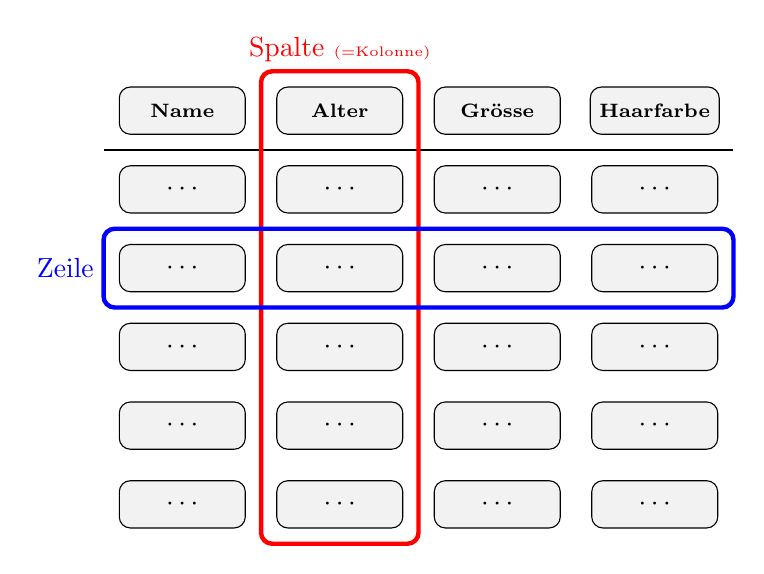
\begin{tikzpicture}
  % Define style for cell
  \tikzstyle{cell} = [draw, rectangle, minimum width=1.6cm, minimum height=.6cm, fill=gray!10, rounded corners]
  \tikzstyle{cellcdot} = [draw, rectangle, minimum width=1.6cm, minimum height=.6cm, fill=gray!0, rounded corners]

  % Draw the table
  \foreach \row in {1,...,6} {
    \foreach \col/\ctitle in {1/Name,2/Alter,3/Grösse,4/Haarfarbe} {
      \node(\col\row)[cell] at (\col*2, -\row) {
      \ifnum\row=1 
      	\scriptsize\textbf{\ctitle}\normalsize
      \else 
      	$\cdots$ 
      \fi
      };
    }
  }
  \draw[black, thick] (1,-1.5) -- (9,-1.5);
  
  \draw [red,ultra thick,rounded corners]
    (3,-.5) rectangle (5,-6.5);

  \draw [blue,ultra thick,rounded corners]
    (1,-2.5) rectangle (9,-3.5);
    
  \node[above] at (4,-0.5){\textcolor{red}{Spalte \tiny(=Kolonne)\normalsize}};
  \node[left] at (1,-3){\textcolor{blue}{Zeile}};
\end{tikzpicture}
}

\begin{frame}[fragile]{Typische Tabellenstruktur}
\highlightTable{1}{1}{1}
\end{frame}


\begin{frame}[fragile]{Typische Tabellenstruktur}
\begin{tikzpicture}
\node (table) {
\tiny
\begin{tabular}{p{.9cm}|p{.9cm}|p{.9cm}|p{.9cm}|p{.9cm}|p{.9cm}|p{.9cm}|p{.9cm}}
  
      \textbf{Name} & \textbf{Ort} & \textbf{Leiter} & \textbf{Lehrer} & \textbf{Schüler} & \textbf{Klassen} & \textbf{Budget}  & ...\\
      \hline
      Maple & Stadt A & H. Peter & 30 & 500 & 20 & 1'000'000 & ...\\
      \hline
  	  Pineview & Stadt B & Fr. Meier & 25 & 450 & 18 & 800'000 & ...\\
      \hline
      Oakridge & Stadt C & H. Smith & 20 & 300 & 12 & 500'000 & ...\\
      \hline
      Elmwood & Stadt D & Fr. Davis & 15 & 350 & 15 & 600'000 & ...\\
      \hline
      ... &... &... &... &... & ... & ... & ...\\
    \end{tabular} 
};

\draw [red,ultra thick]
  ($(table.south west) !1/6*3! (table.north west)$)
  rectangle 
  ($(table.south east) !1/6*4! (table.north east)$);
  
\draw [blue,ultra thick]
  ($(table.south west) !1/8*3! (table.south east)$)
  rectangle 
  ($(table.north west) !1/8*4! (table.north east)$);
\end{tikzpicture}
\end{frame}